\documentclass[11pt,a4paper]{article}
\usepackage[utf8]{inputenc}
\usepackage{amsmath}
\usepackage{amsfonts}
\usepackage{amssymb}
\usepackage{pdfpages}
\usepackage{graphicx}
\graphicspath{{./Img/}}
\begin{document}
\begin{titlepage}
   \begin{center}
       \vspace*{1cm}
 
       \textbf{LIVEtheMUSIC}
 
       \vspace{0.5cm}
        Software requirement specification
 
       \vspace{5cm}
 
       \textbf{Daniele Ferrarelli, Marco Ferri, Lorenzo Valeriani}
 
       \vfill
   \end{center}
\end{titlepage}
\section{Introduction}
\subsection{Aim of the document}
The aim of this document is to present a description of “LIVE the MUSIC”. It will present the purpose and features of the system and what the system will do.
\subsection{Overview of the defined system}
This system allows the user to remain updated about music events in the area according to the user’s musical taste. It will present detailed information about the location and transportation methods. The service allows the user to discover new artists that s/he may like. The user will be able to know which music events their friends will attend.
\subsection{Operational settings}
“LIVE the MUSIC” should run on any Operating System and browser that supports the Java Environment (version 8 or higher). 
\subsection{Related systems}
Similar services are provided by TicketOne website and Virgin Radio application.
TicketOne: 
The advantage of our system is that it suggests events based on friends’ participation and on specific filters applied by the user. Although does not provide an On-site method to buy the ticket and needs to redirect the user to TicketOne. 
Virgin Radio:
Our system provides social features and the selection of musical events is not limited to rock events. One disadvantage of our system is that relies on artists to add music events to the service.
\section{User Stories}
\subsection{Ferrarelli}
\begin{itemize}
\item As an artist, I want to create an artist’s profile, so that I can post news about me.
\item As an artist, I want to add music events to the service, so that I can advertise my events.
\item As a user, I want to see which music event my friends are going to attend, so that I can join them.
\end{itemize}
\subsection{Ferri}
\begin{itemize}
\item As a user, I want to add other users to my friend list, so that I can see their activities.
\item As a traveler, I want a map of the area where the music event will take place, so that I can
find bus stops or train stations.
\item As a user, I want a news section for the artists I follow, so that I can stay updated.
\end{itemize}
\subsection{Valeriani}
\begin{itemize}
\item As an artist, I want to post news on the system, so that I can keep my followers updated.
\item As a user, I want to reject a friend request, so that I can enhance my privacy.
\item As a user, I want a list of suggested artists, so that I can discover new artists.
\end{itemize}
\section{Functional Requirements}
\subsection{Ferrarelli}
\begin{itemize}
\item The system shall provide a list of music events hosted in locations in a radius specified by the user.
\item The system shall allow the user to add other users to their friend list.
\item The system shall provide the list of music events attended by the user.
\end{itemize}
\subsection{Ferri}
\begin{itemize}
\item The system shall allow the artist to create a new music event, specifying its name, date and location.
\item The system shall allow the user to view news of their followed artists.
\item The system shall allow the user to remove the participation to a music event, selected by the user.
\end{itemize}
\subsection{Valeriani}
\begin{itemize}
\item The system shall allow the user to search for music events, specifying the artist’s name.
\item The system shall allow the user to add an artist to the list of followed artists.
\item The system shall provide the user with a list of suggested music events, based on their friends' participation.
\end{itemize}
\section{Dictionary}
\begin{itemize}
\item News section: list of news posted by followed artists.
\item Follow: show the news posted by an artist on the user's news section.
\end{itemize}
\section{Use Case Diagram}
\hspace*{-4cm}  
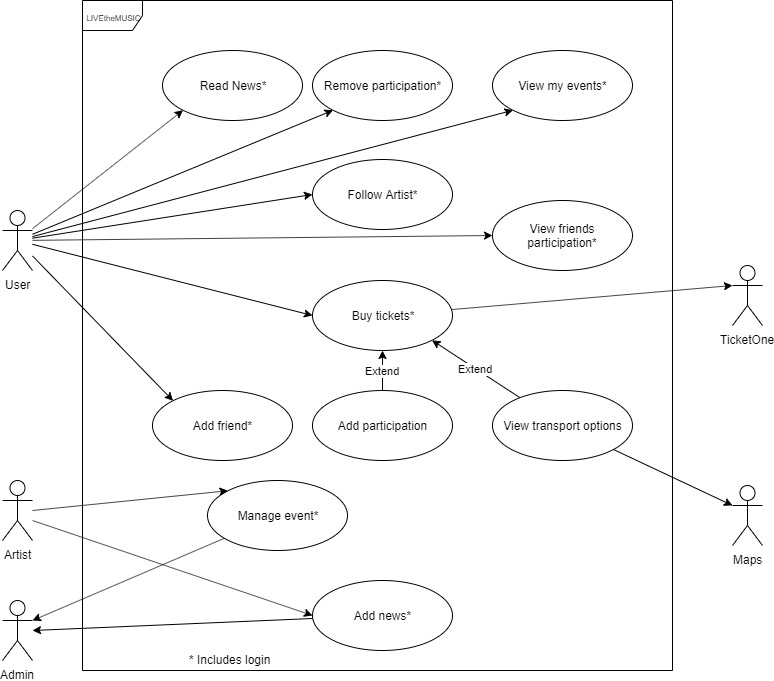
\includegraphics[scale=0.7]{UseCaseFinal.jpg}
\section{Activity Diagram}
\subsection{Ferrarelli}
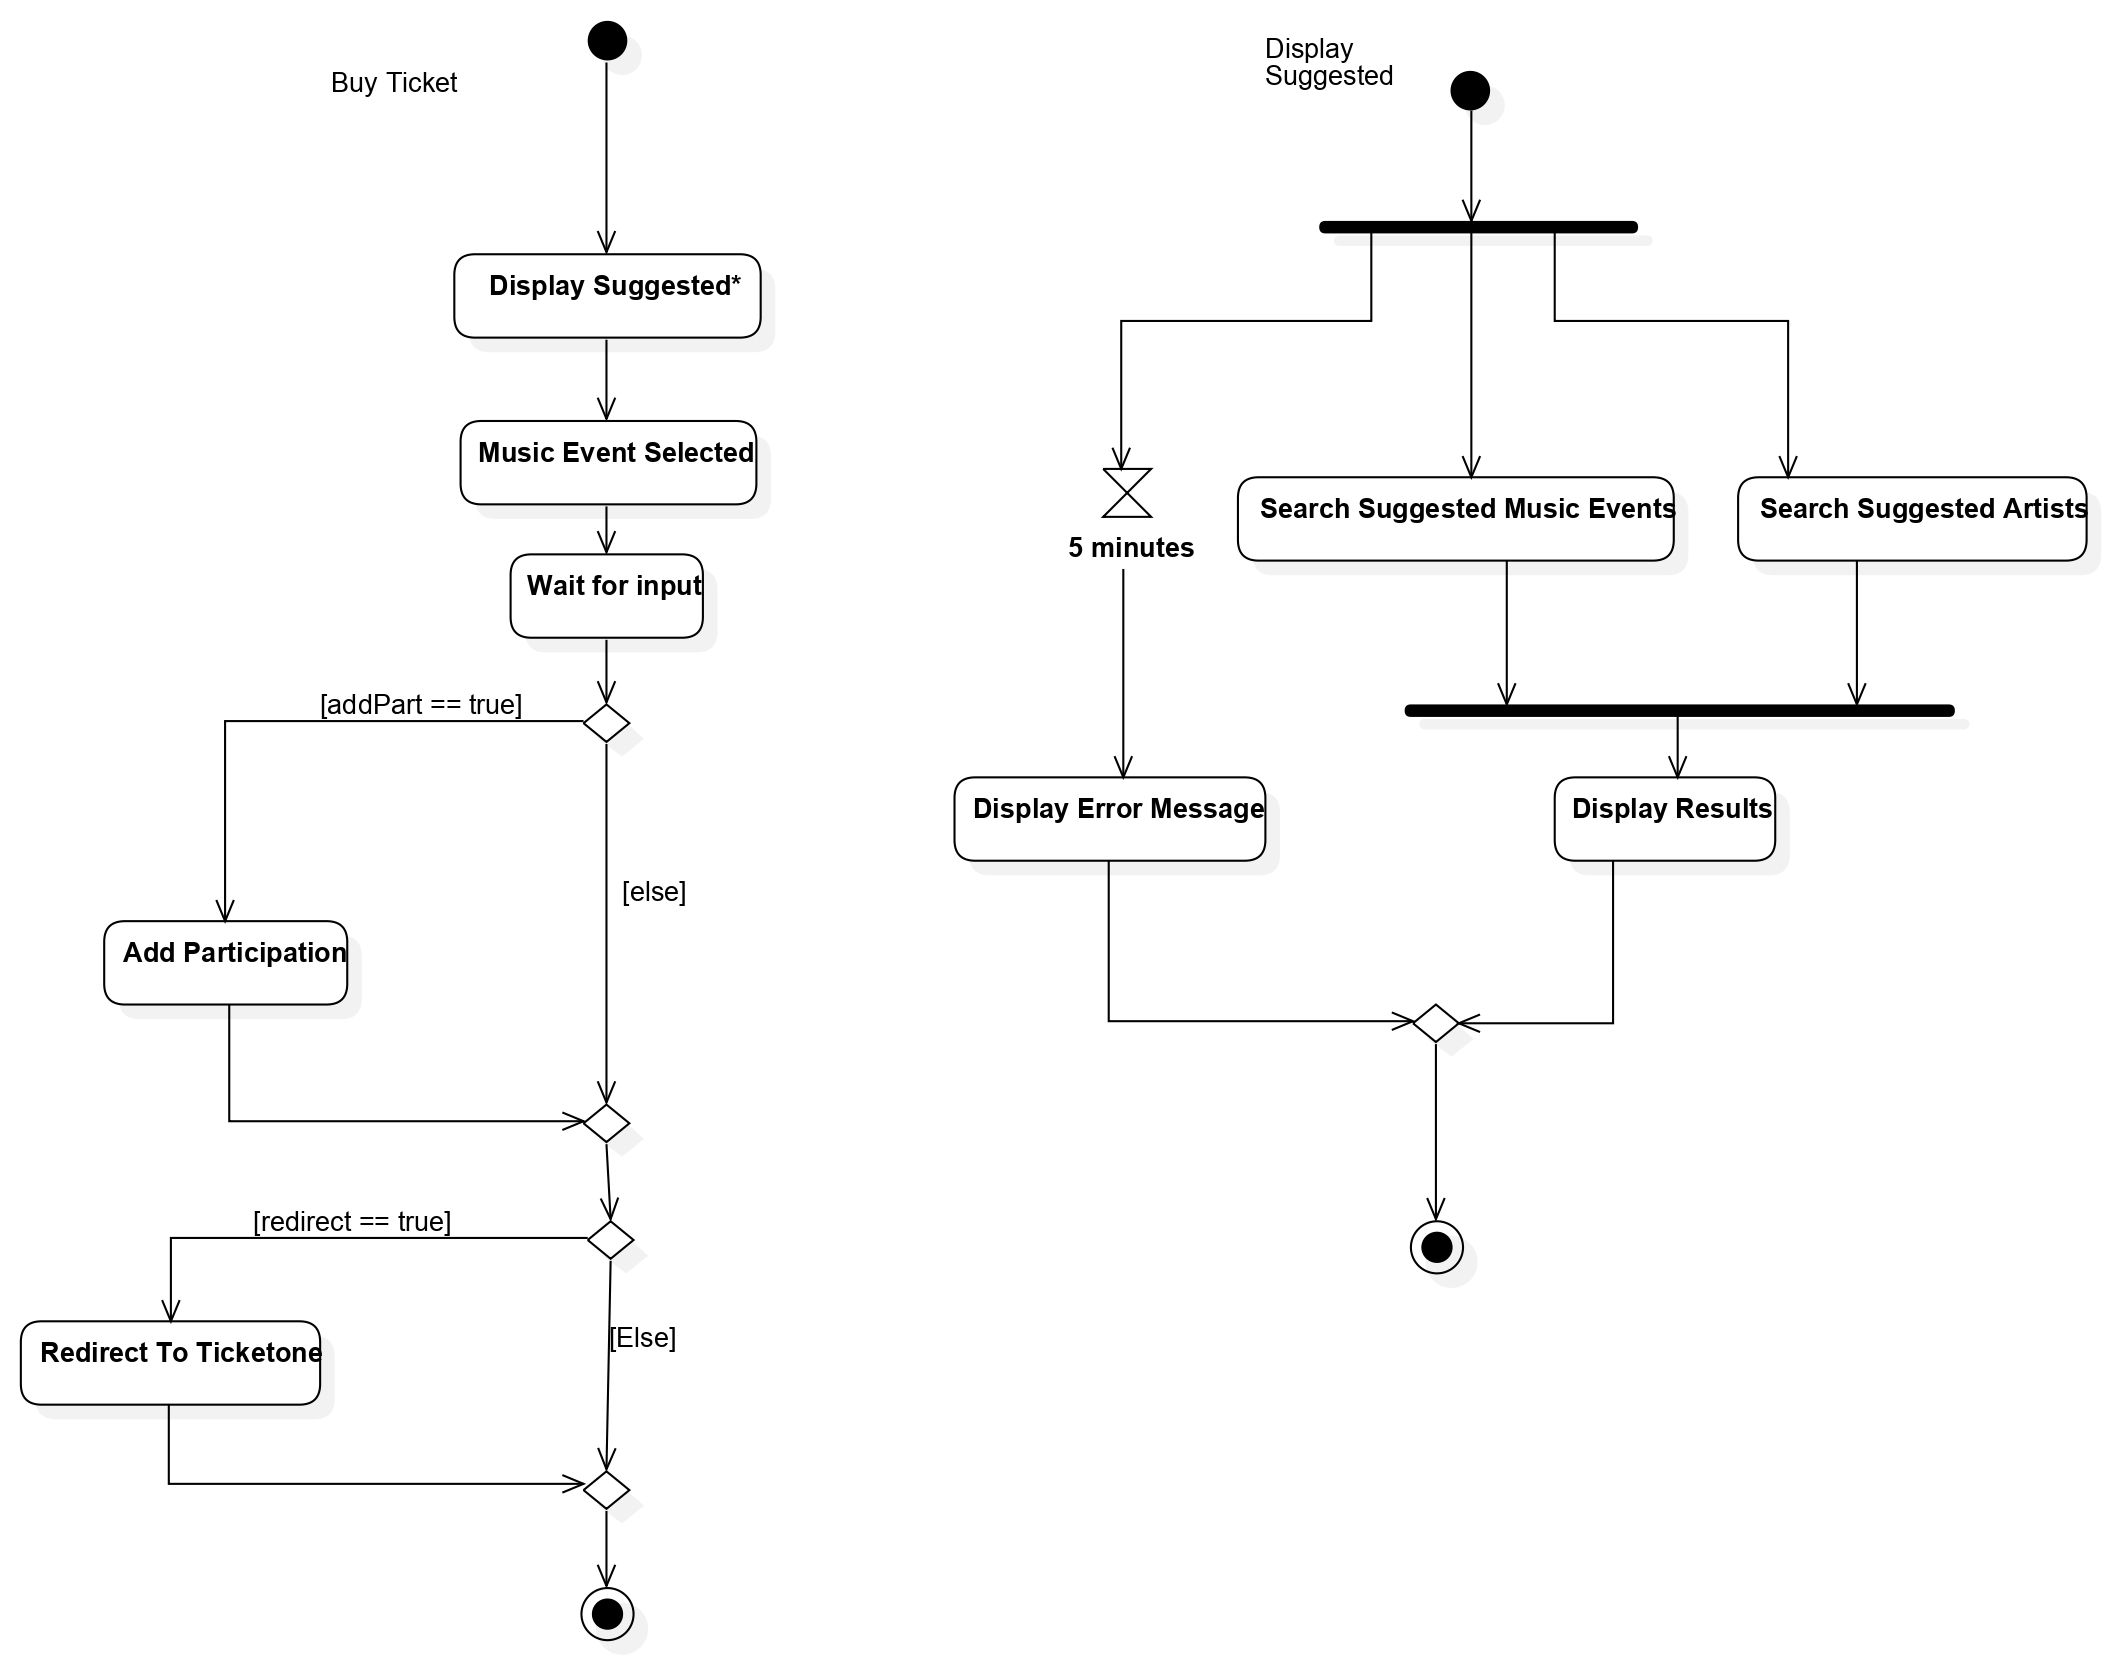
\includegraphics[scale=0.4]{ADFerrarelli.jpg}
\subsection{Ferri}
\subsubsection{}
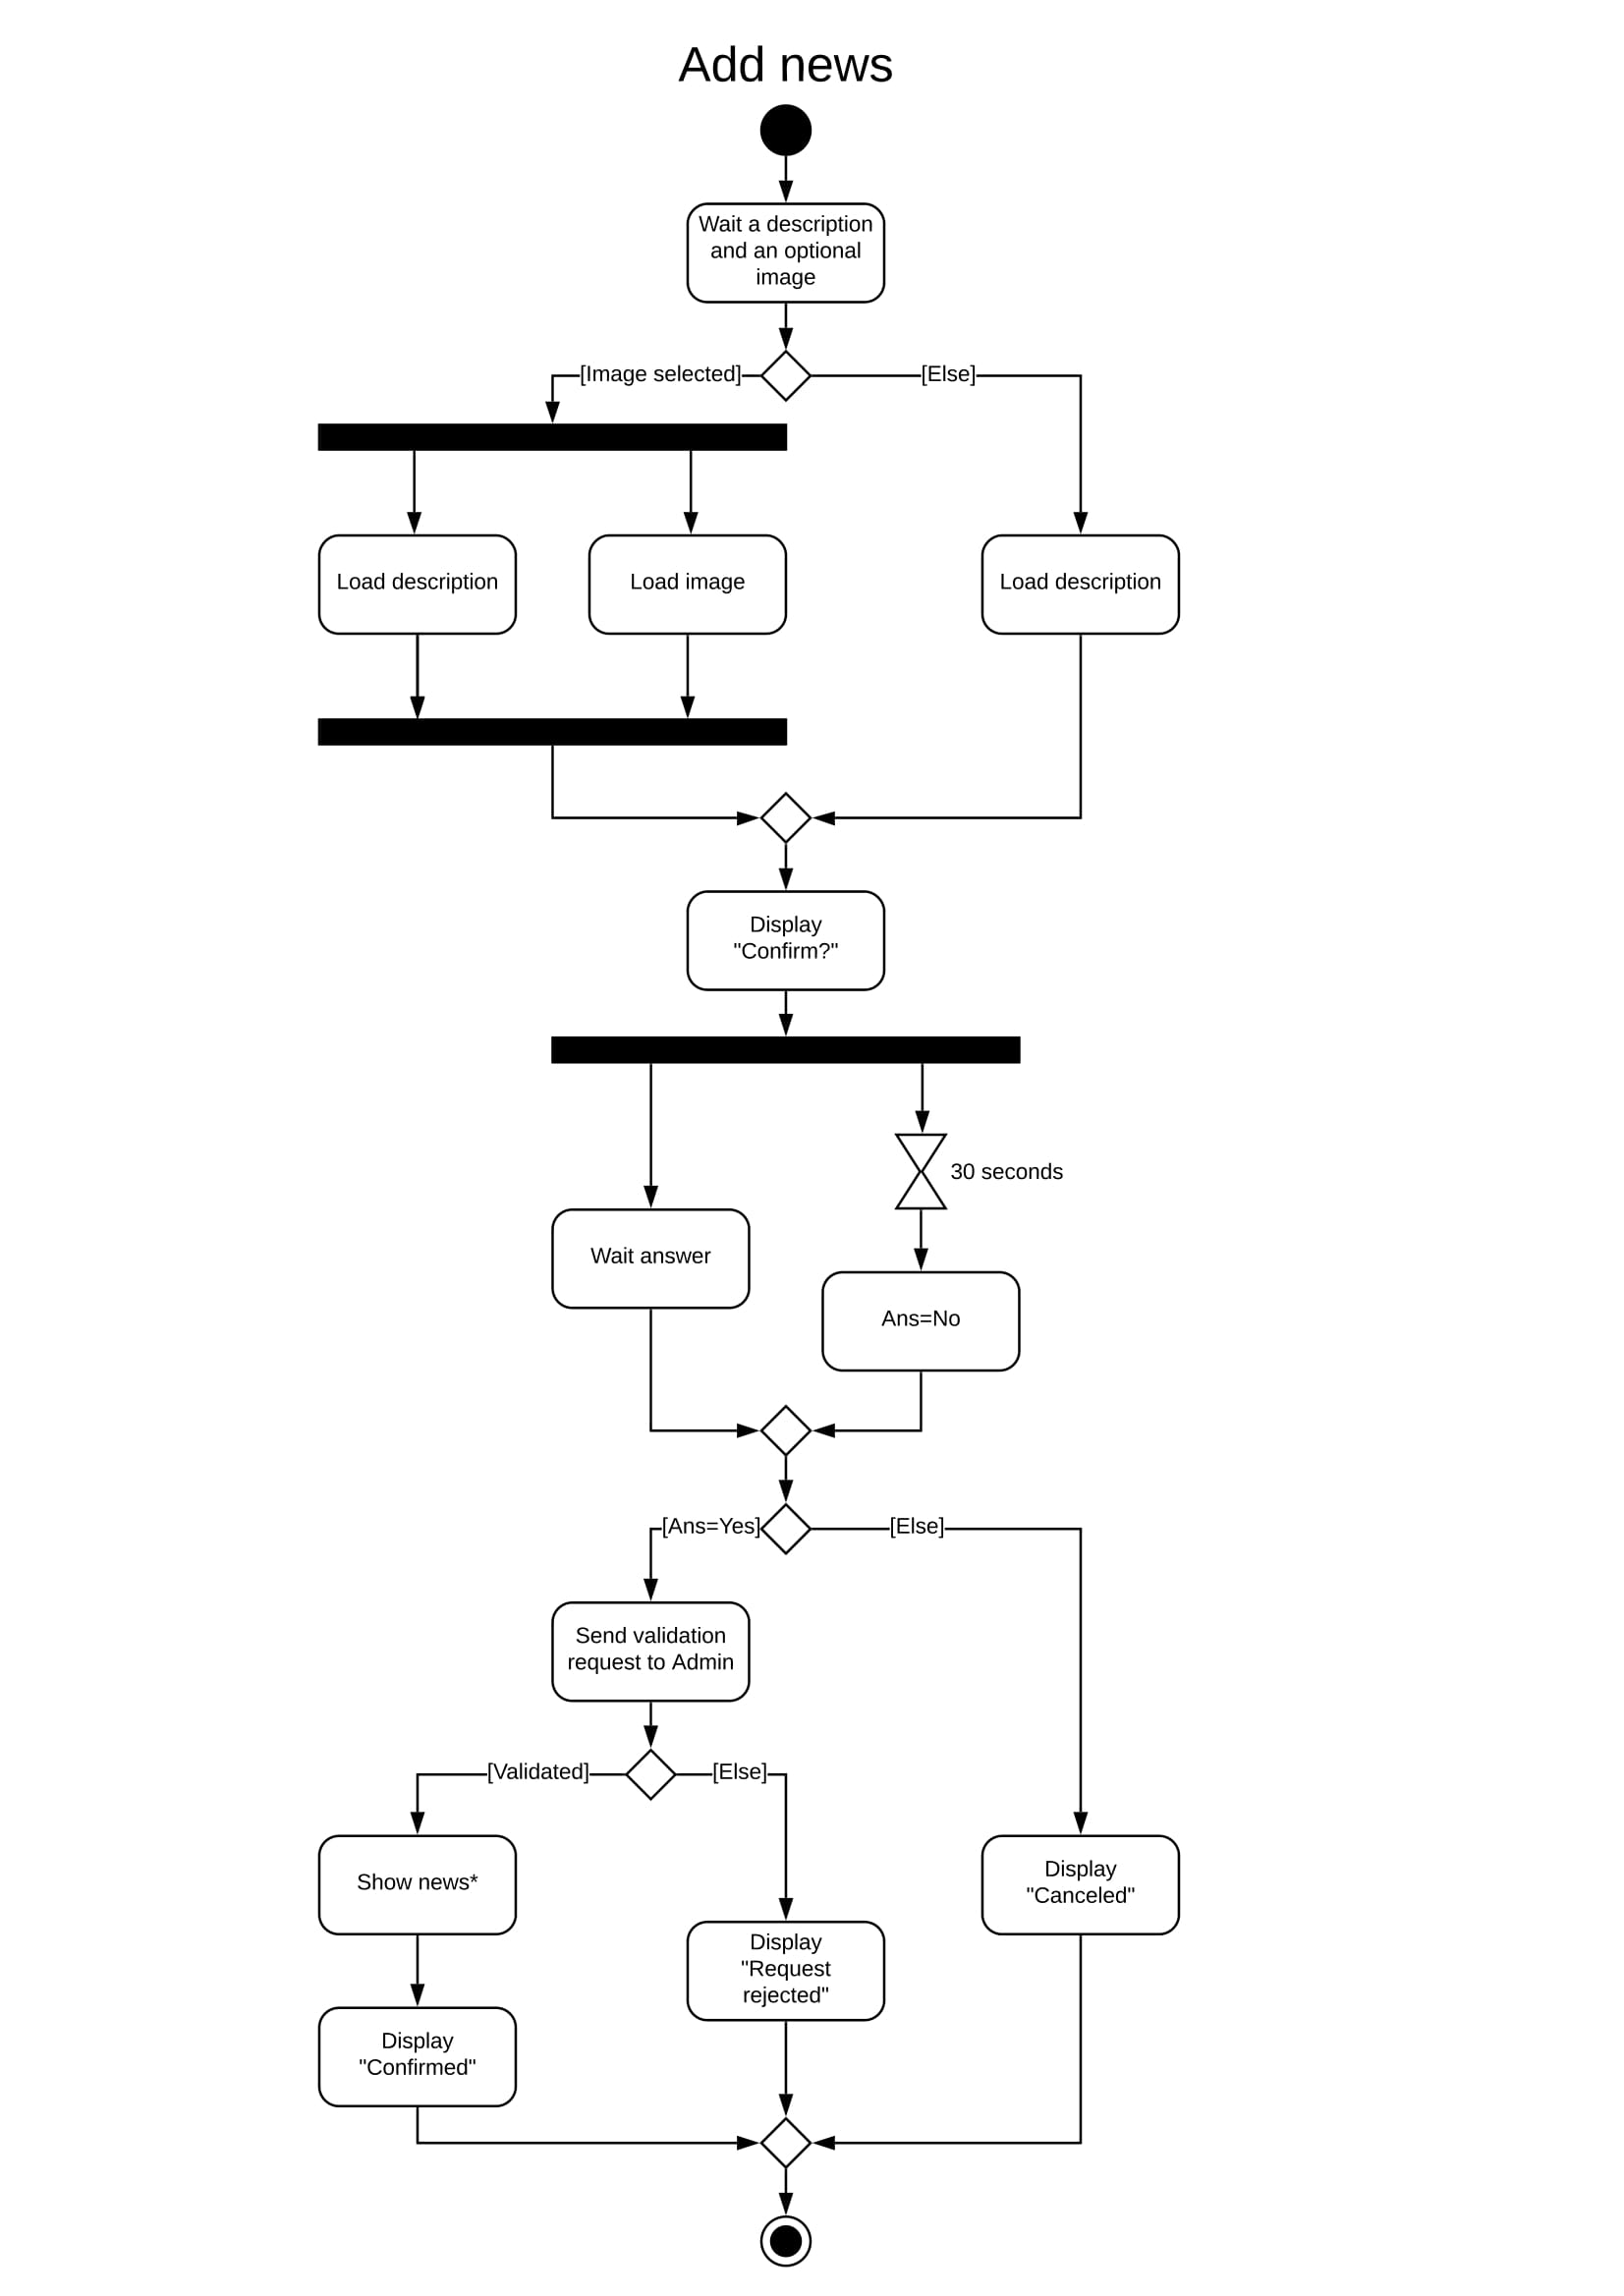
\includegraphics[scale=0.2]{AD1Ferri.jpg}
\subsubsection{}
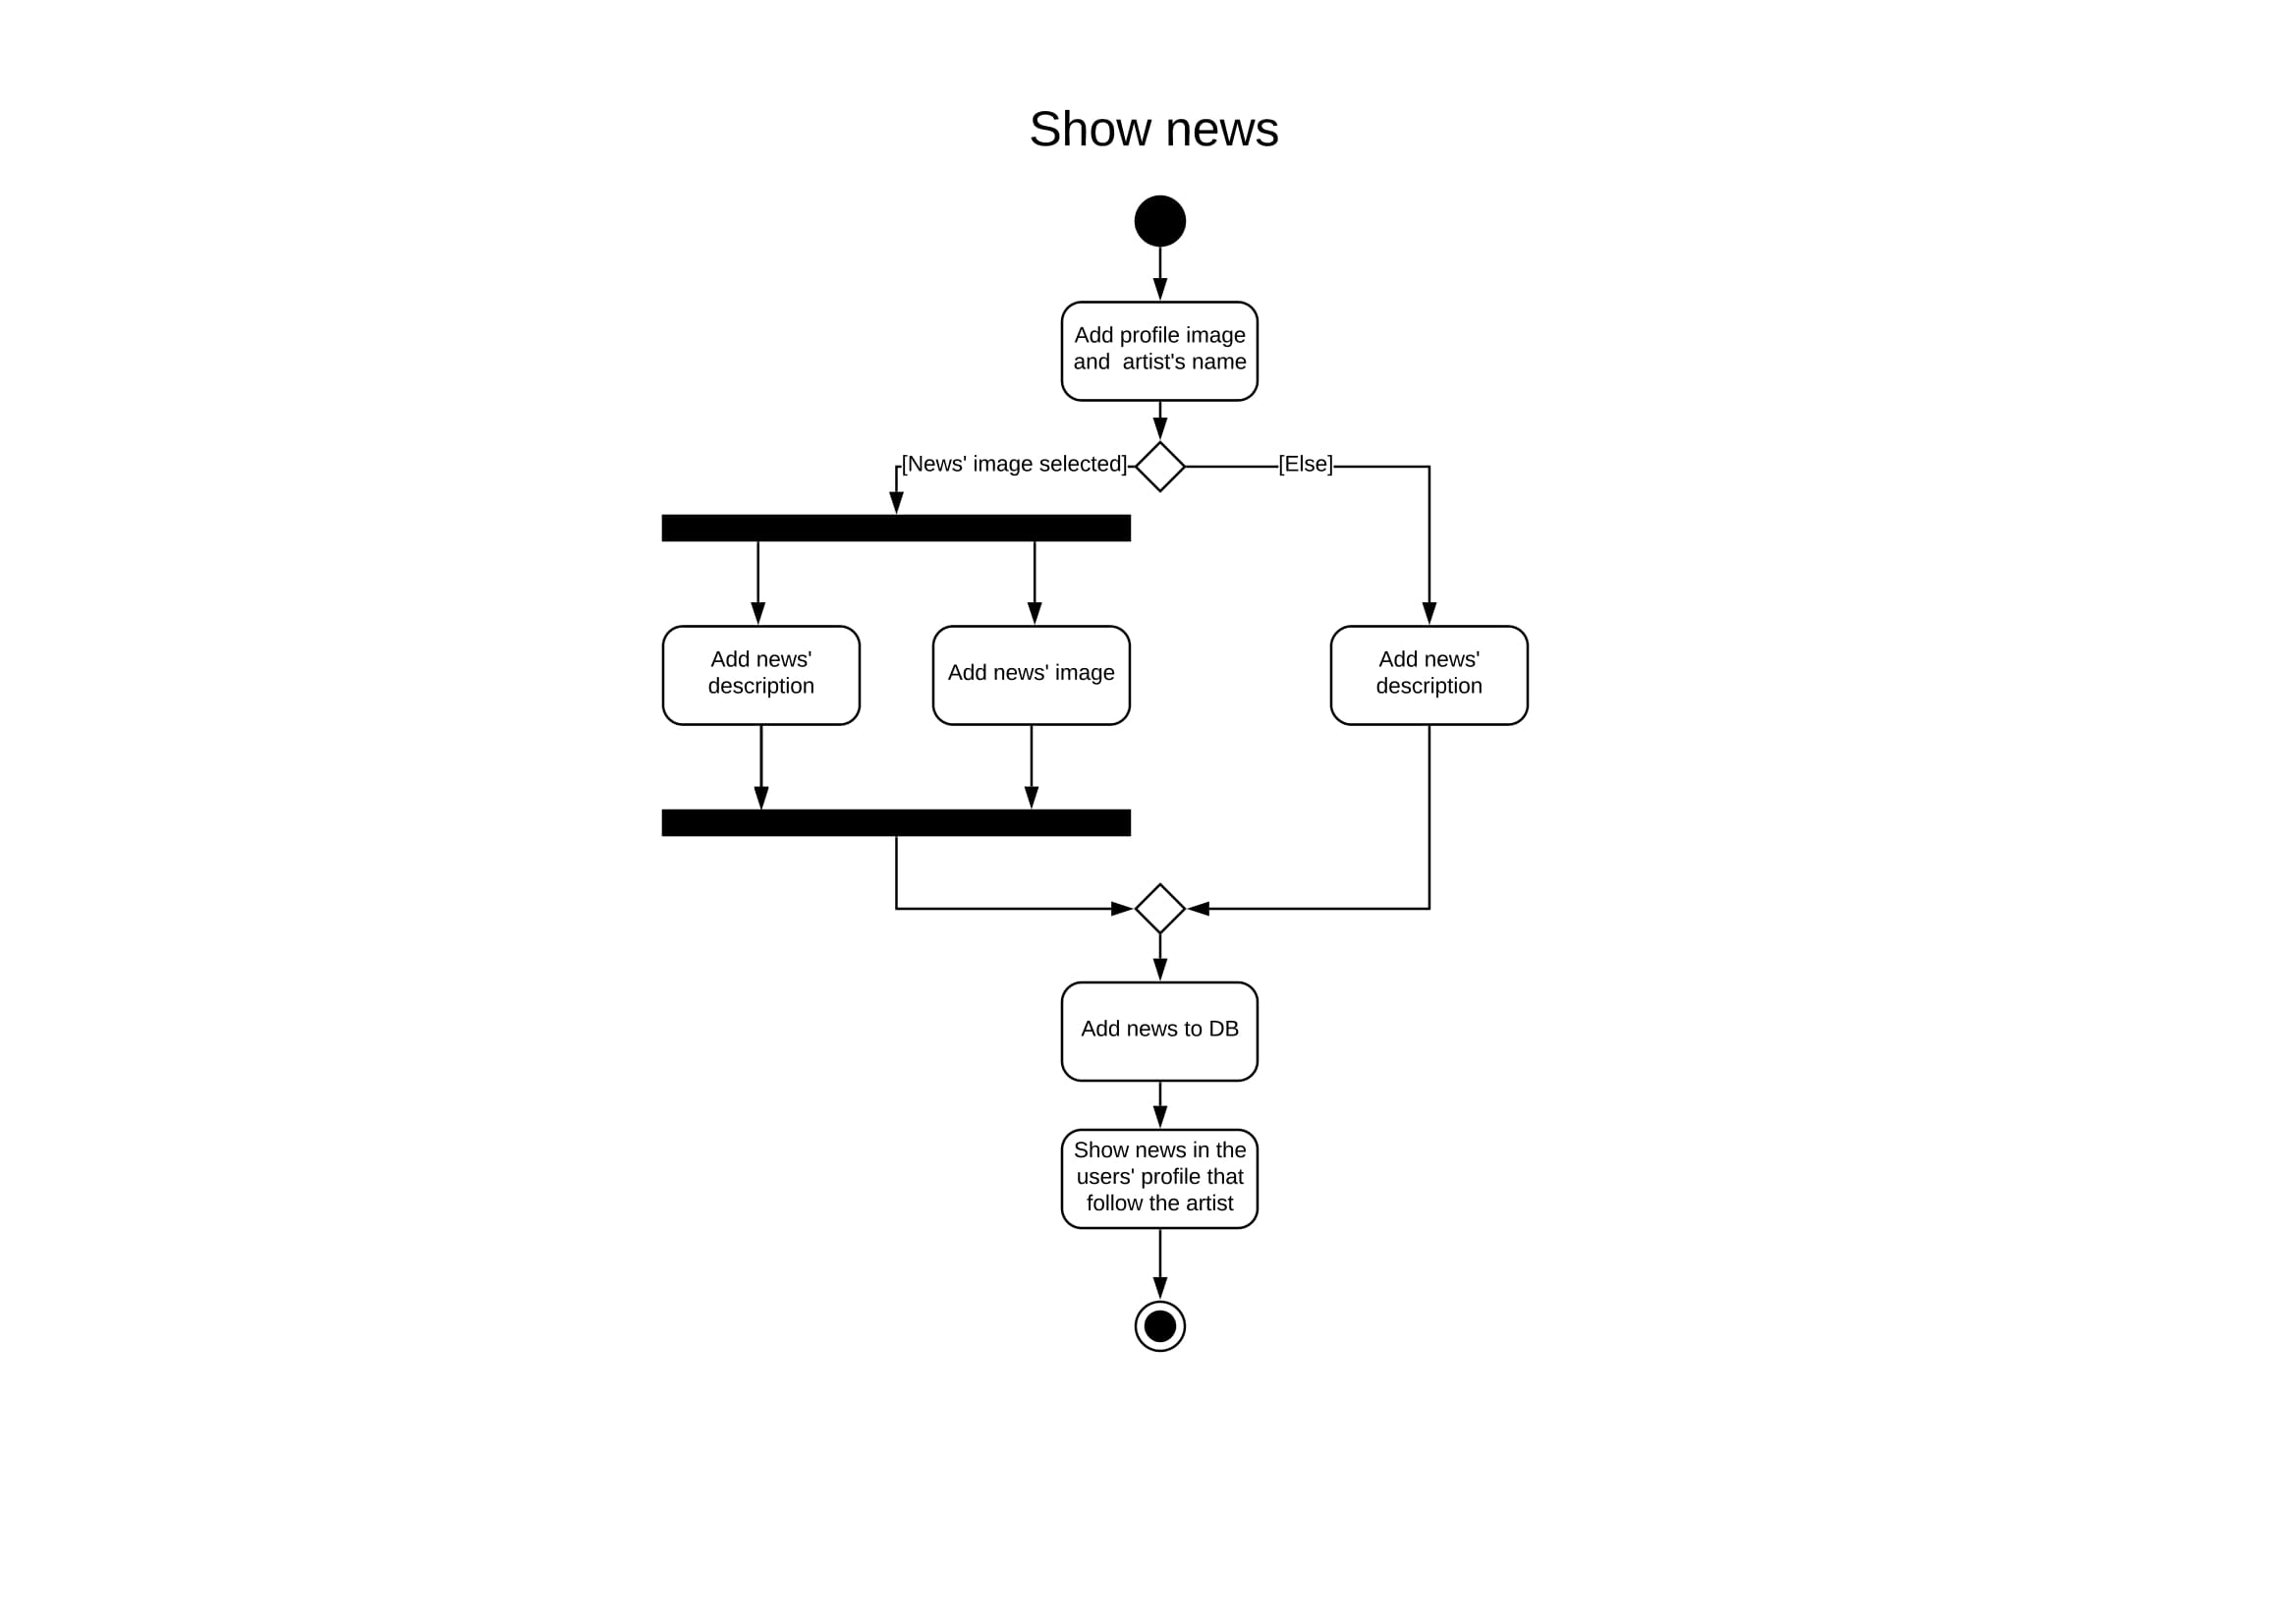
\includegraphics[scale=0.2]{AD2Ferri.jpg}
\subsection{Valeriani}
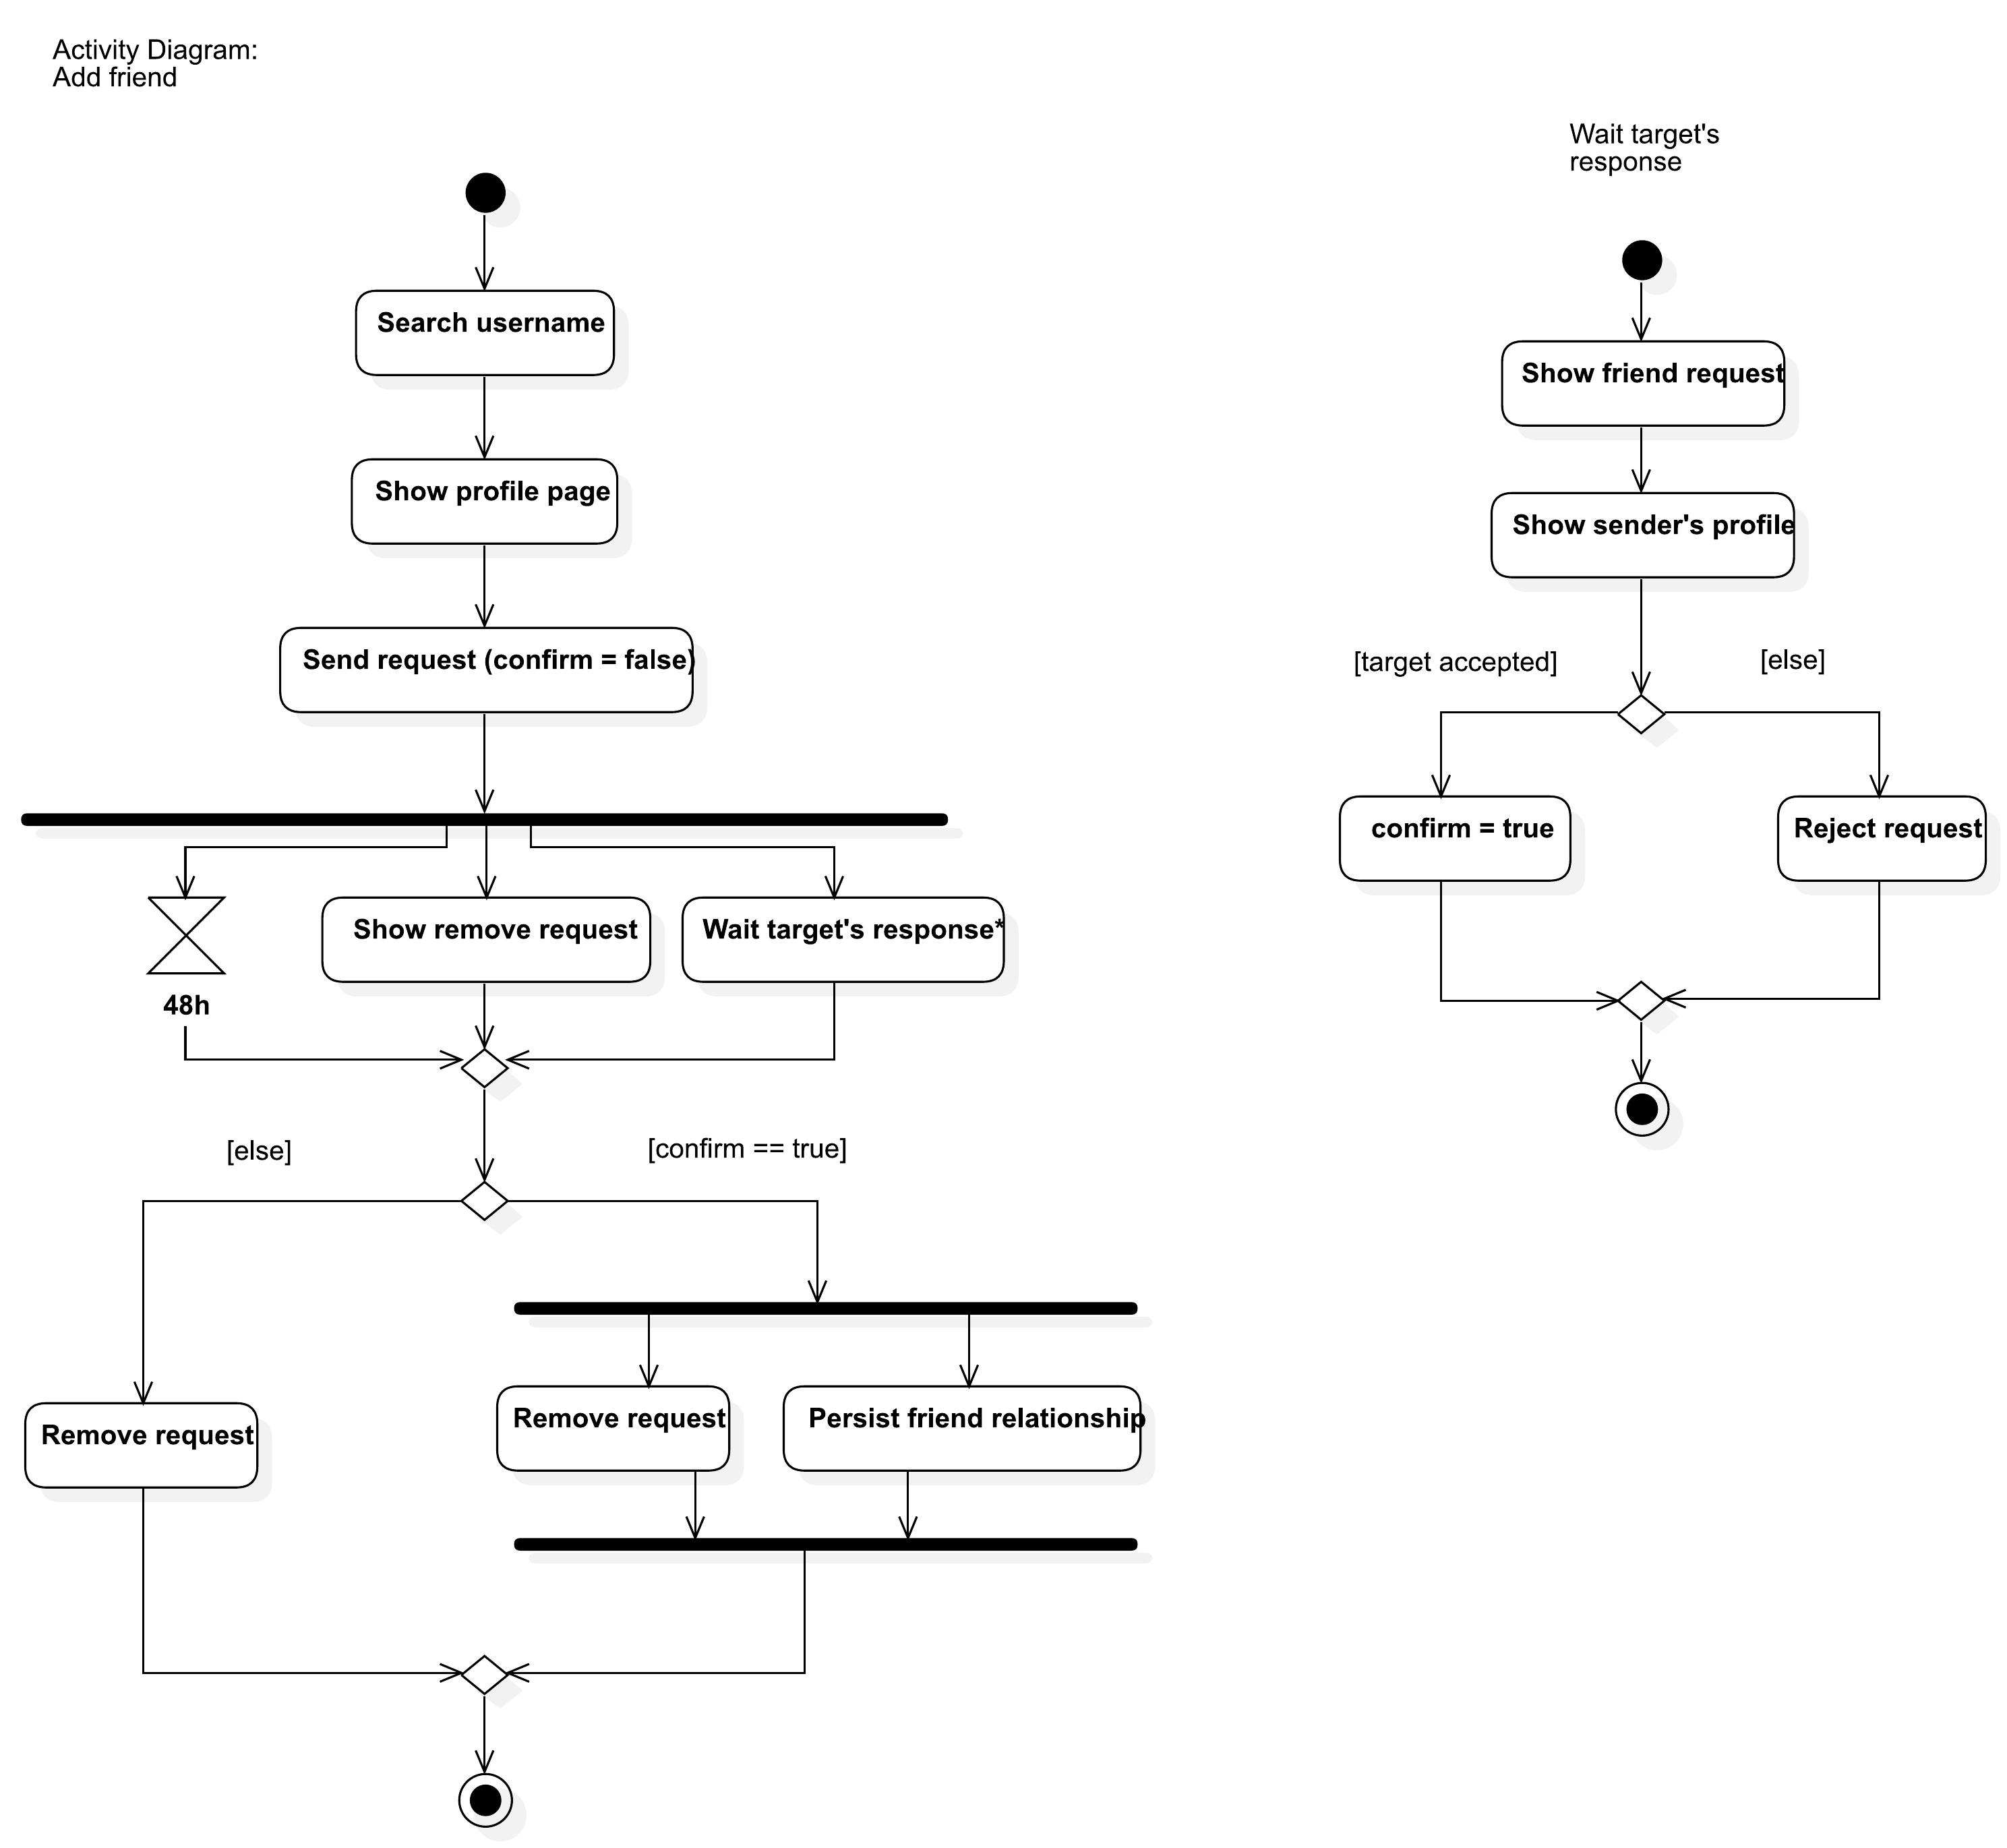
\includegraphics[scale=0.4]{ADValeriani.jpg}
\subsection{Extra}
\section{Sequence Diagram}
\subsection{Ferrarelli}
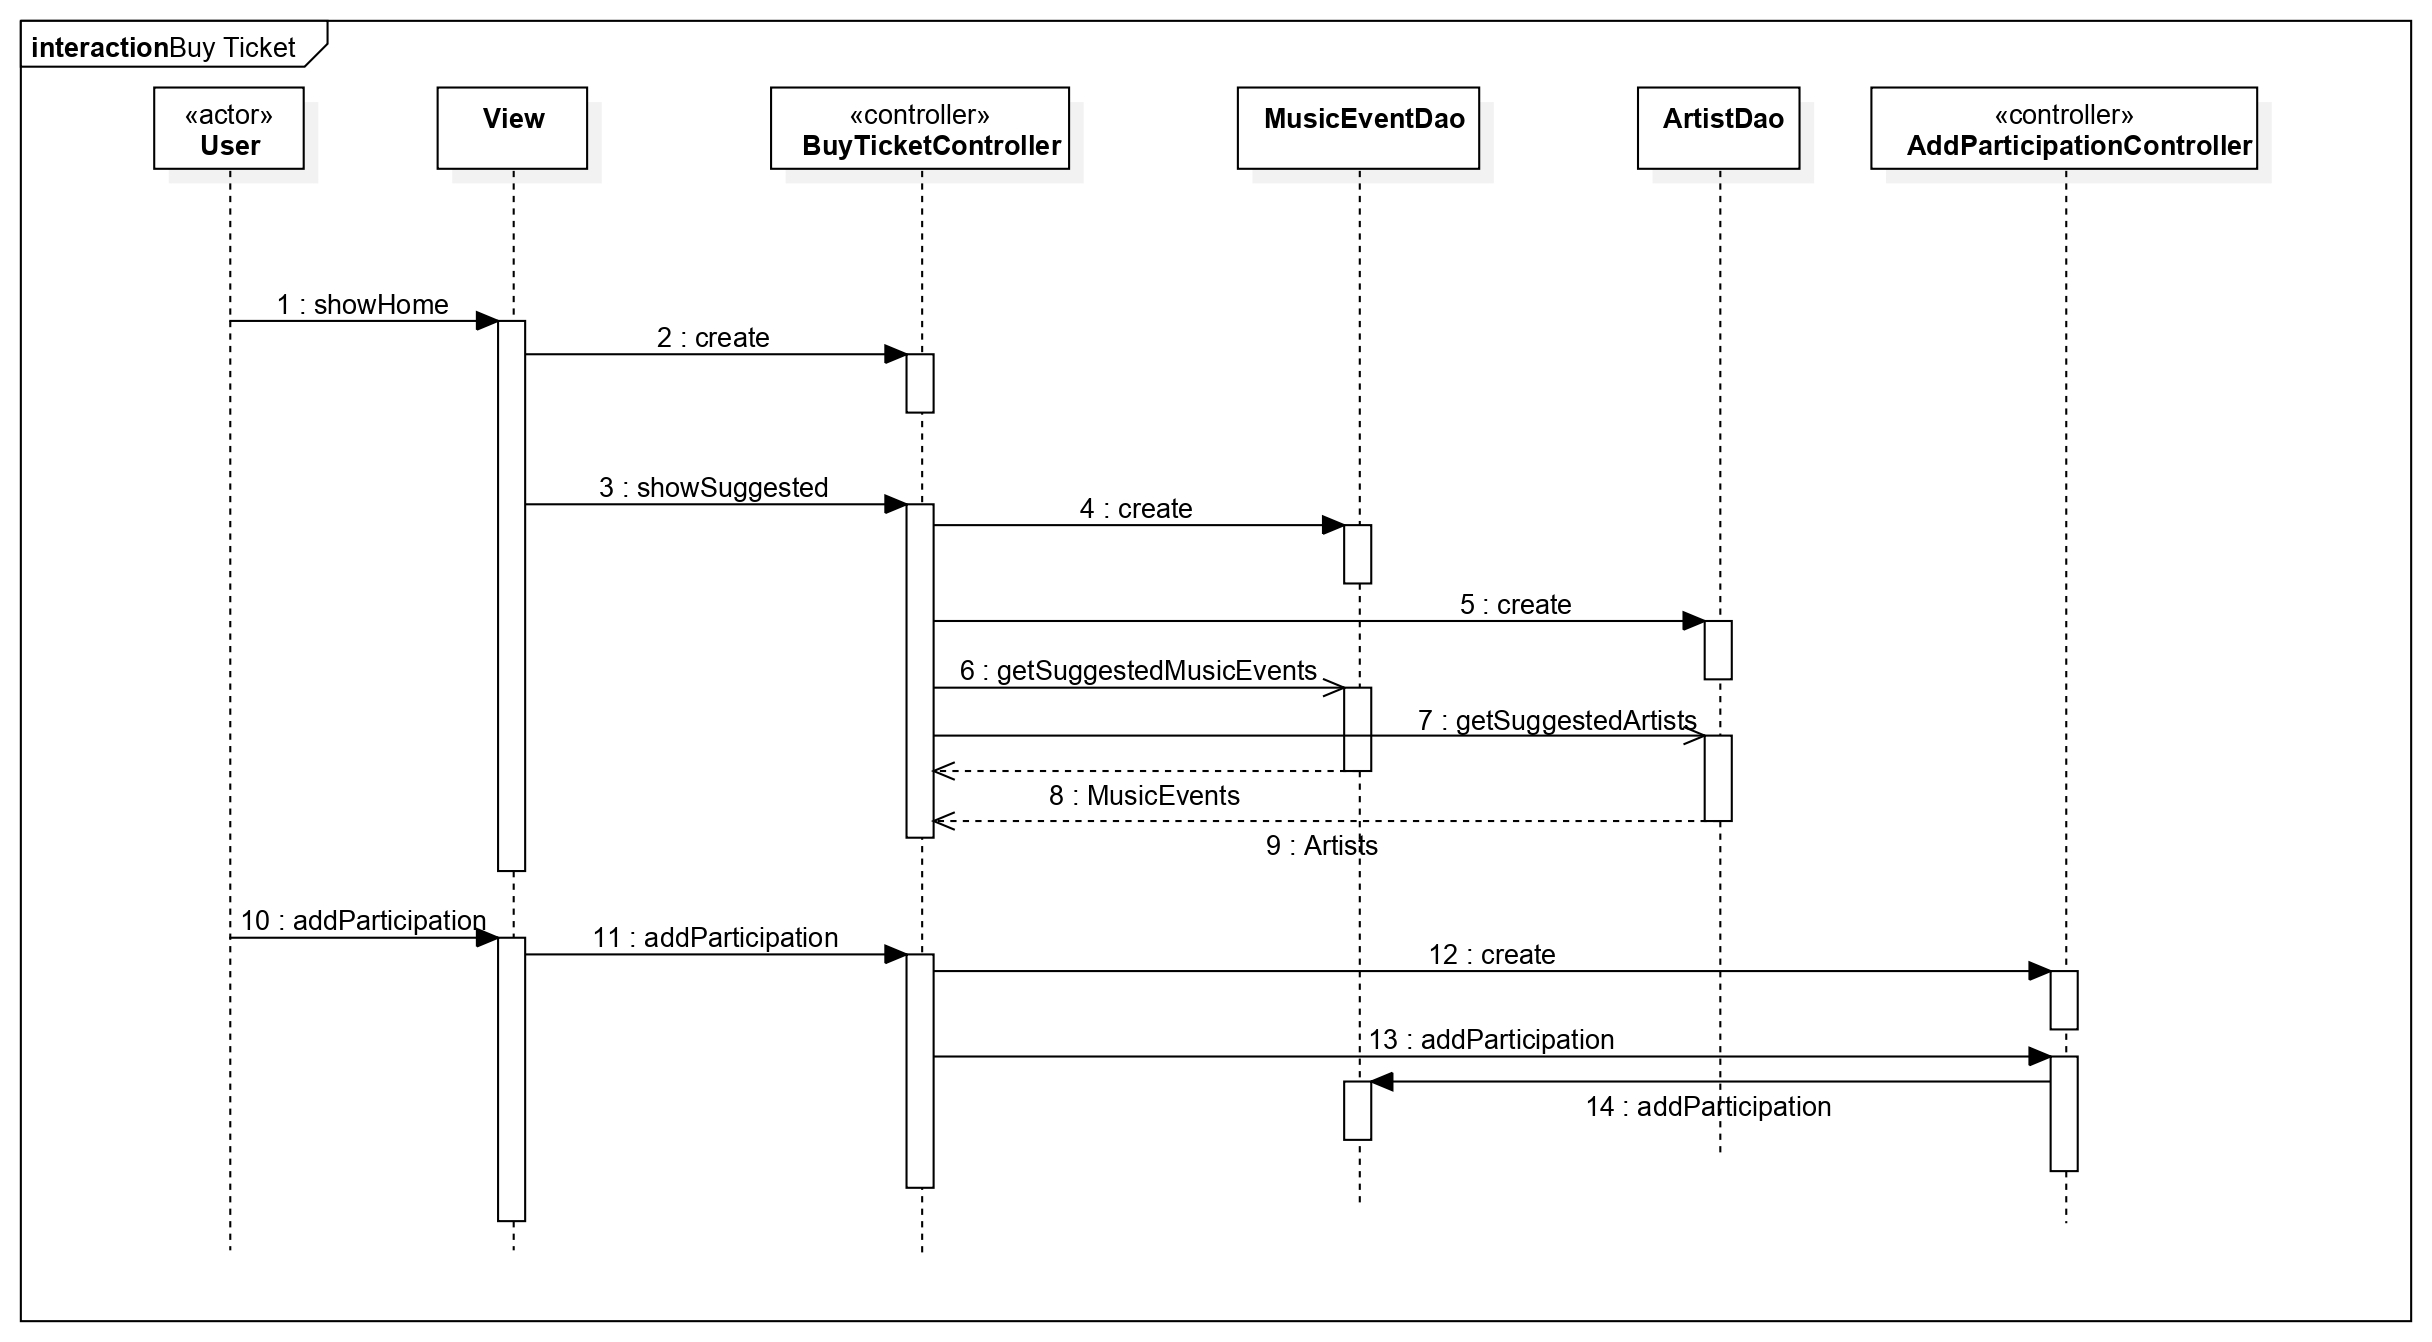
\includegraphics[scale=0.4]{SQFerrarelli.jpg}
\subsection{Ferri}
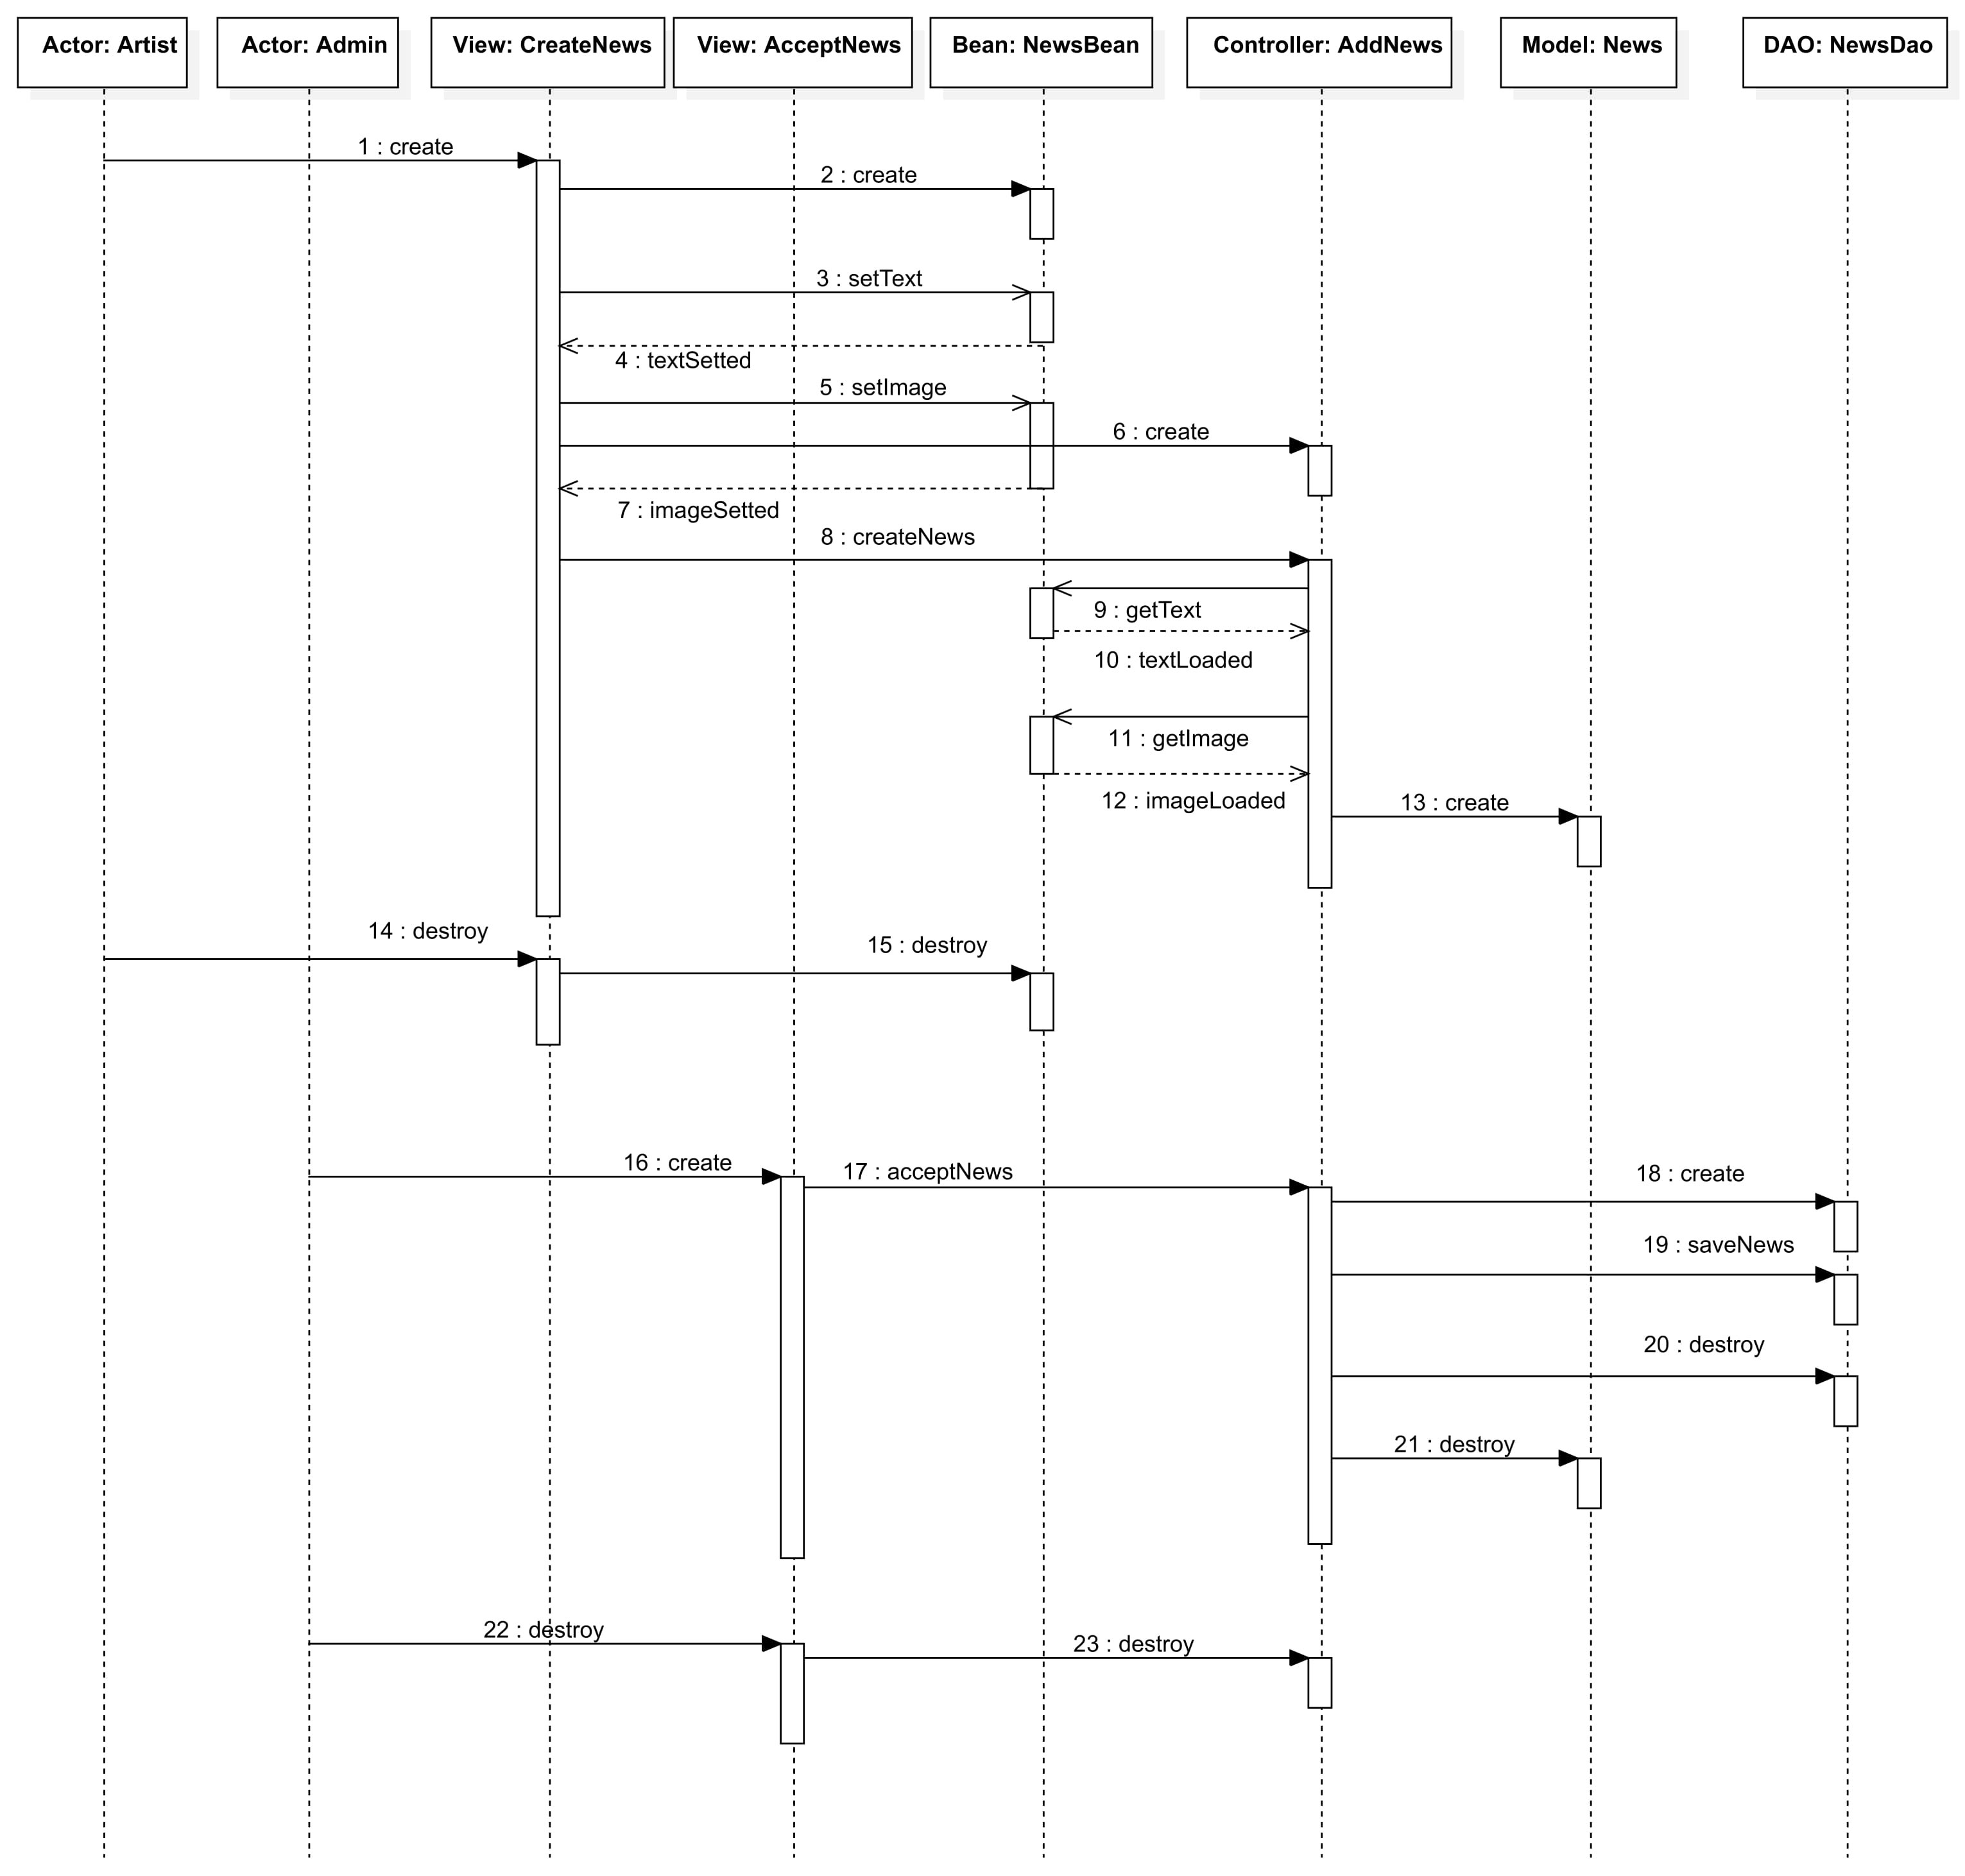
\includegraphics[scale=0.15]{SQFerri.jpg}
\subsection{Valeriani}
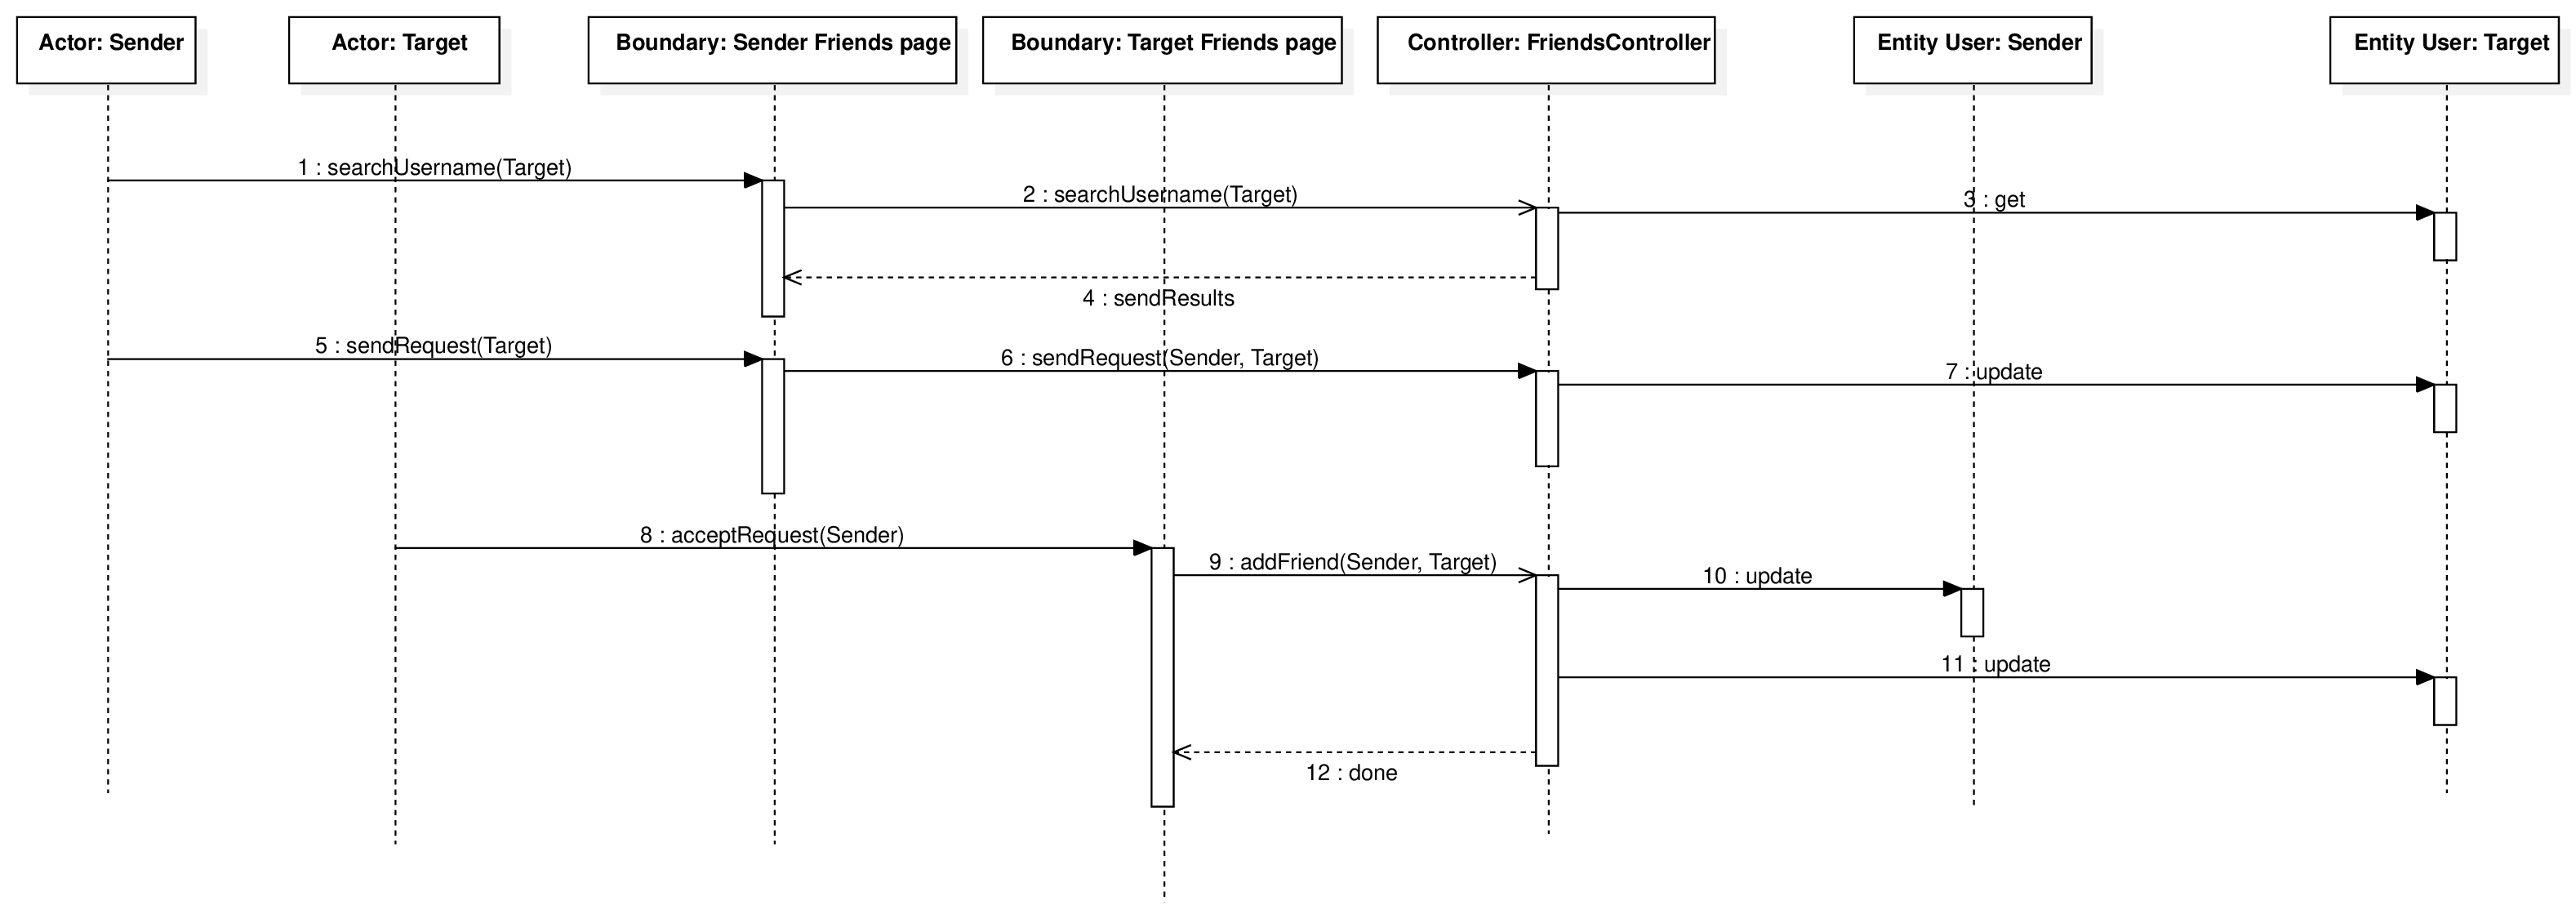
\includegraphics[scale=0.14]{SQValeriani.jpg}
\section{State Diagram}
\subsection{Ferrarelli}
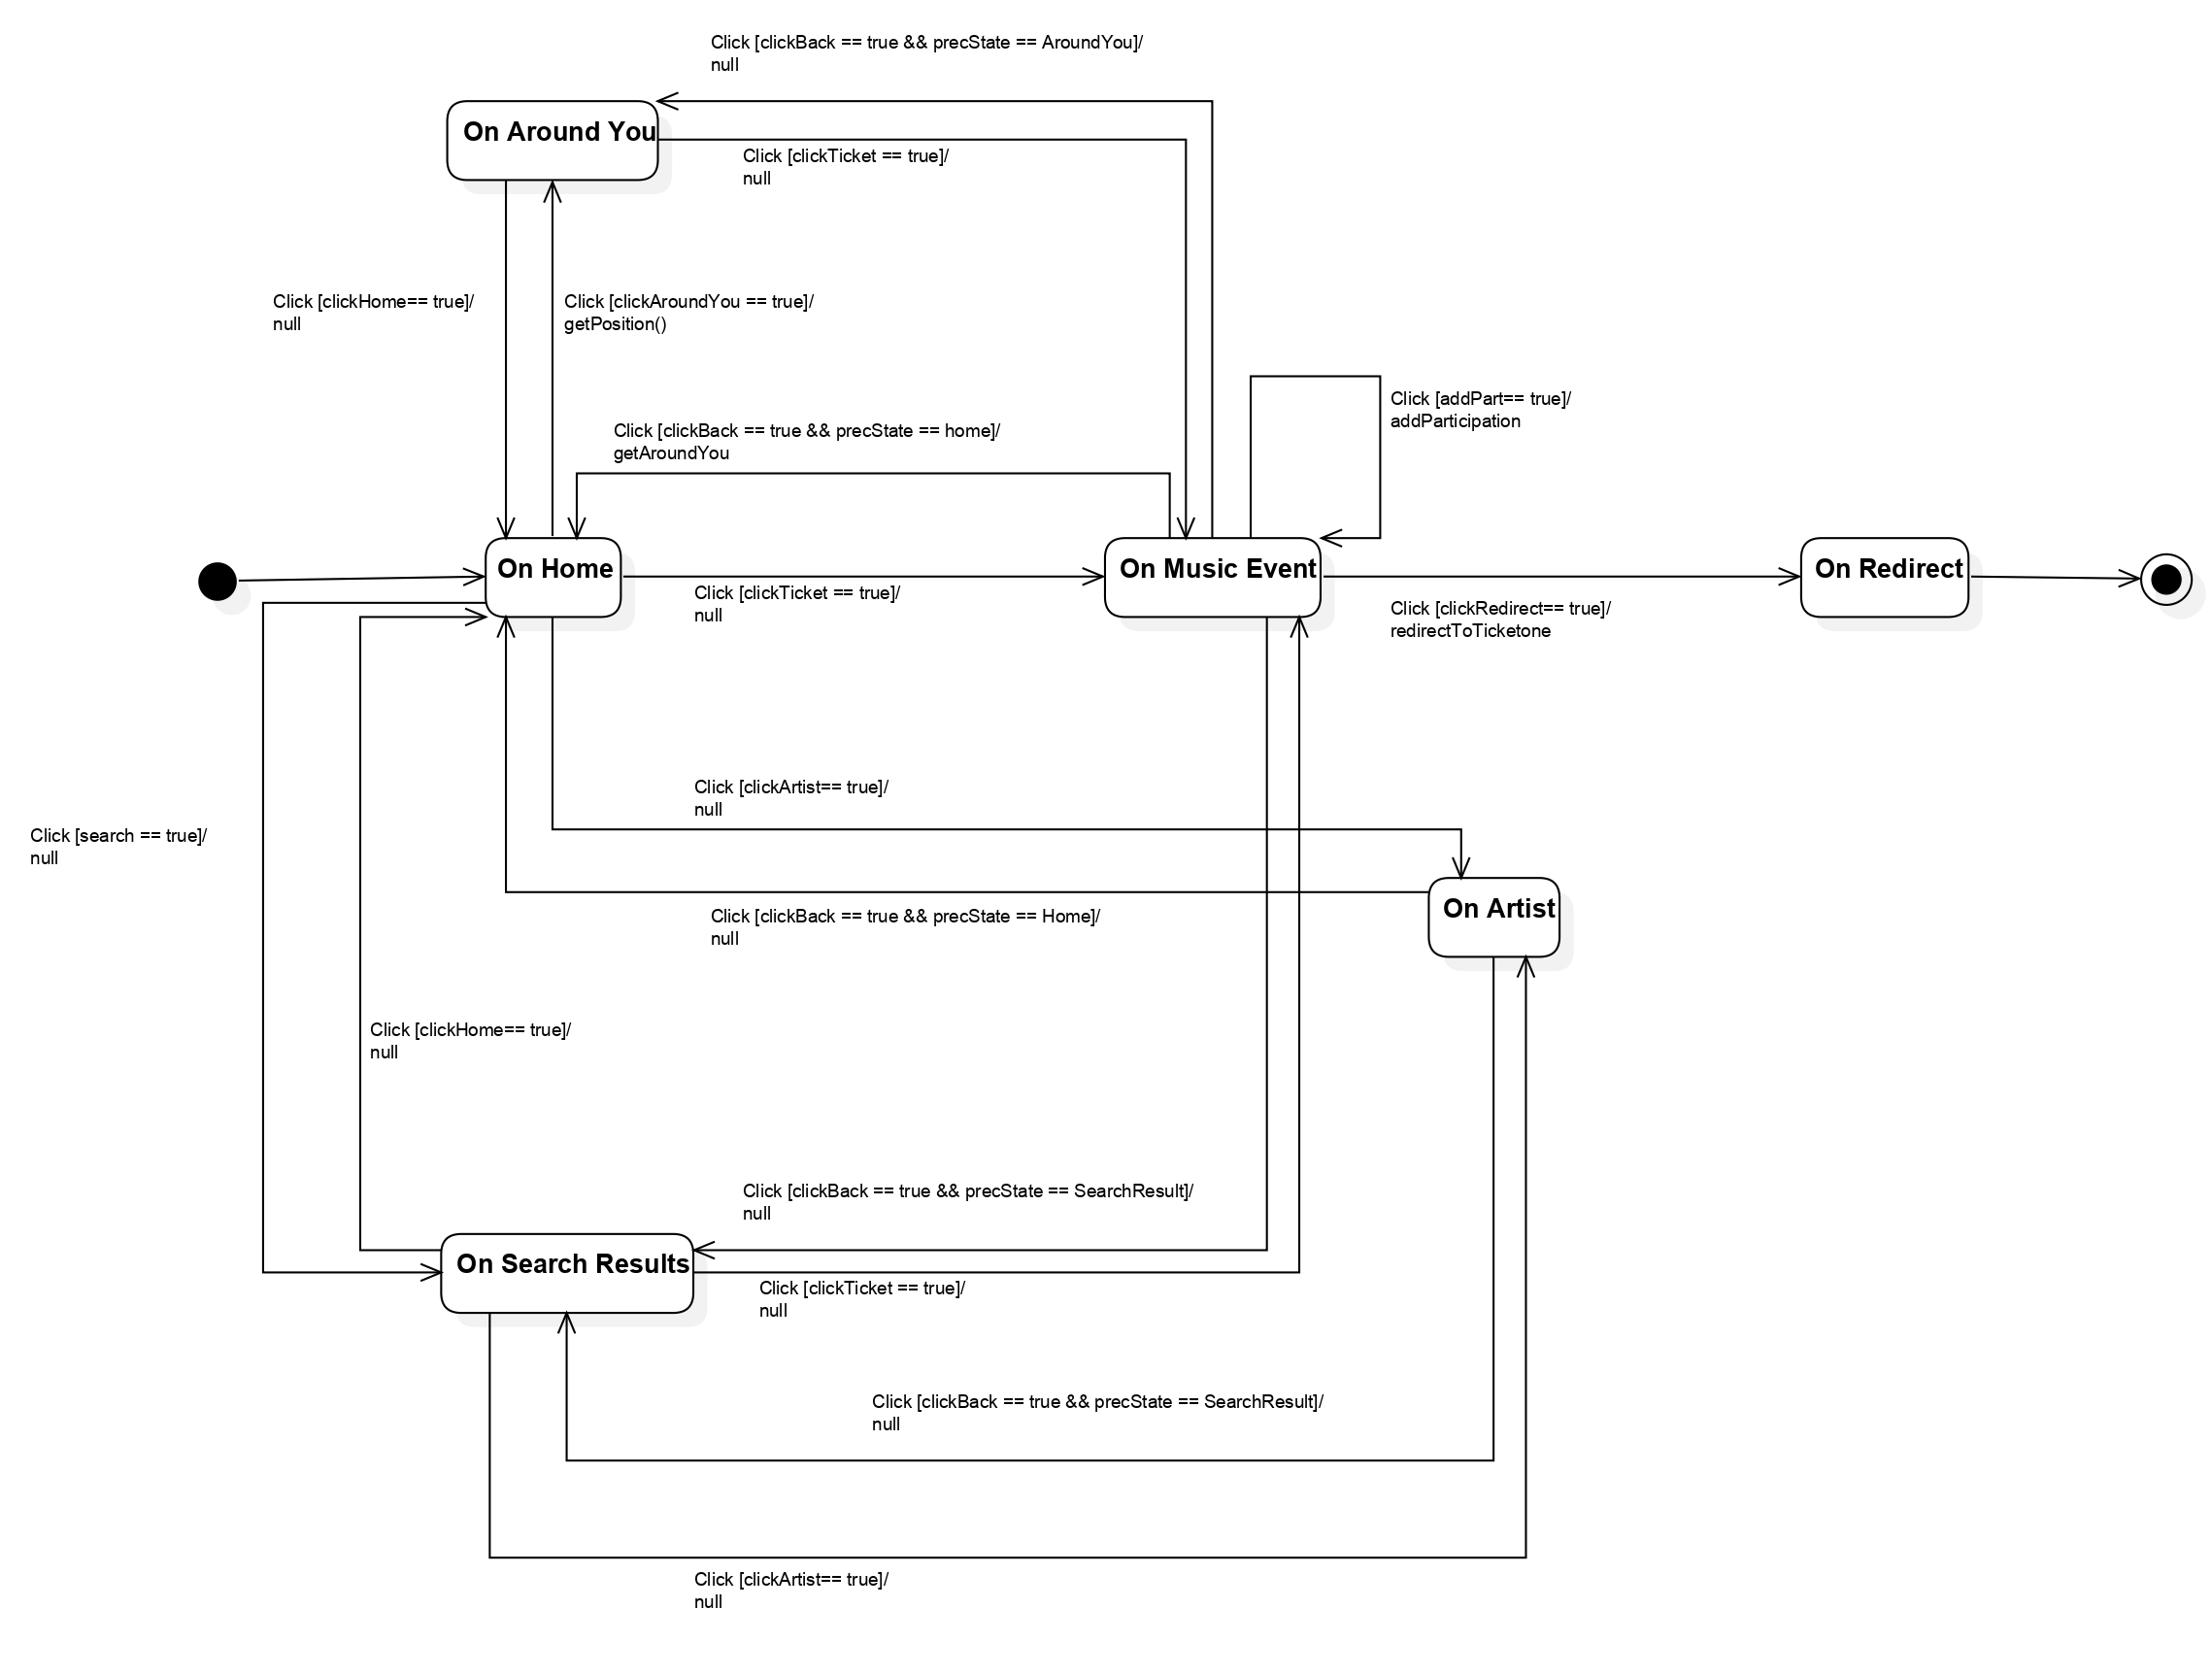
\includegraphics[scale=0.4]{SDFerrarelli.jpg}
\subsection{Ferri}
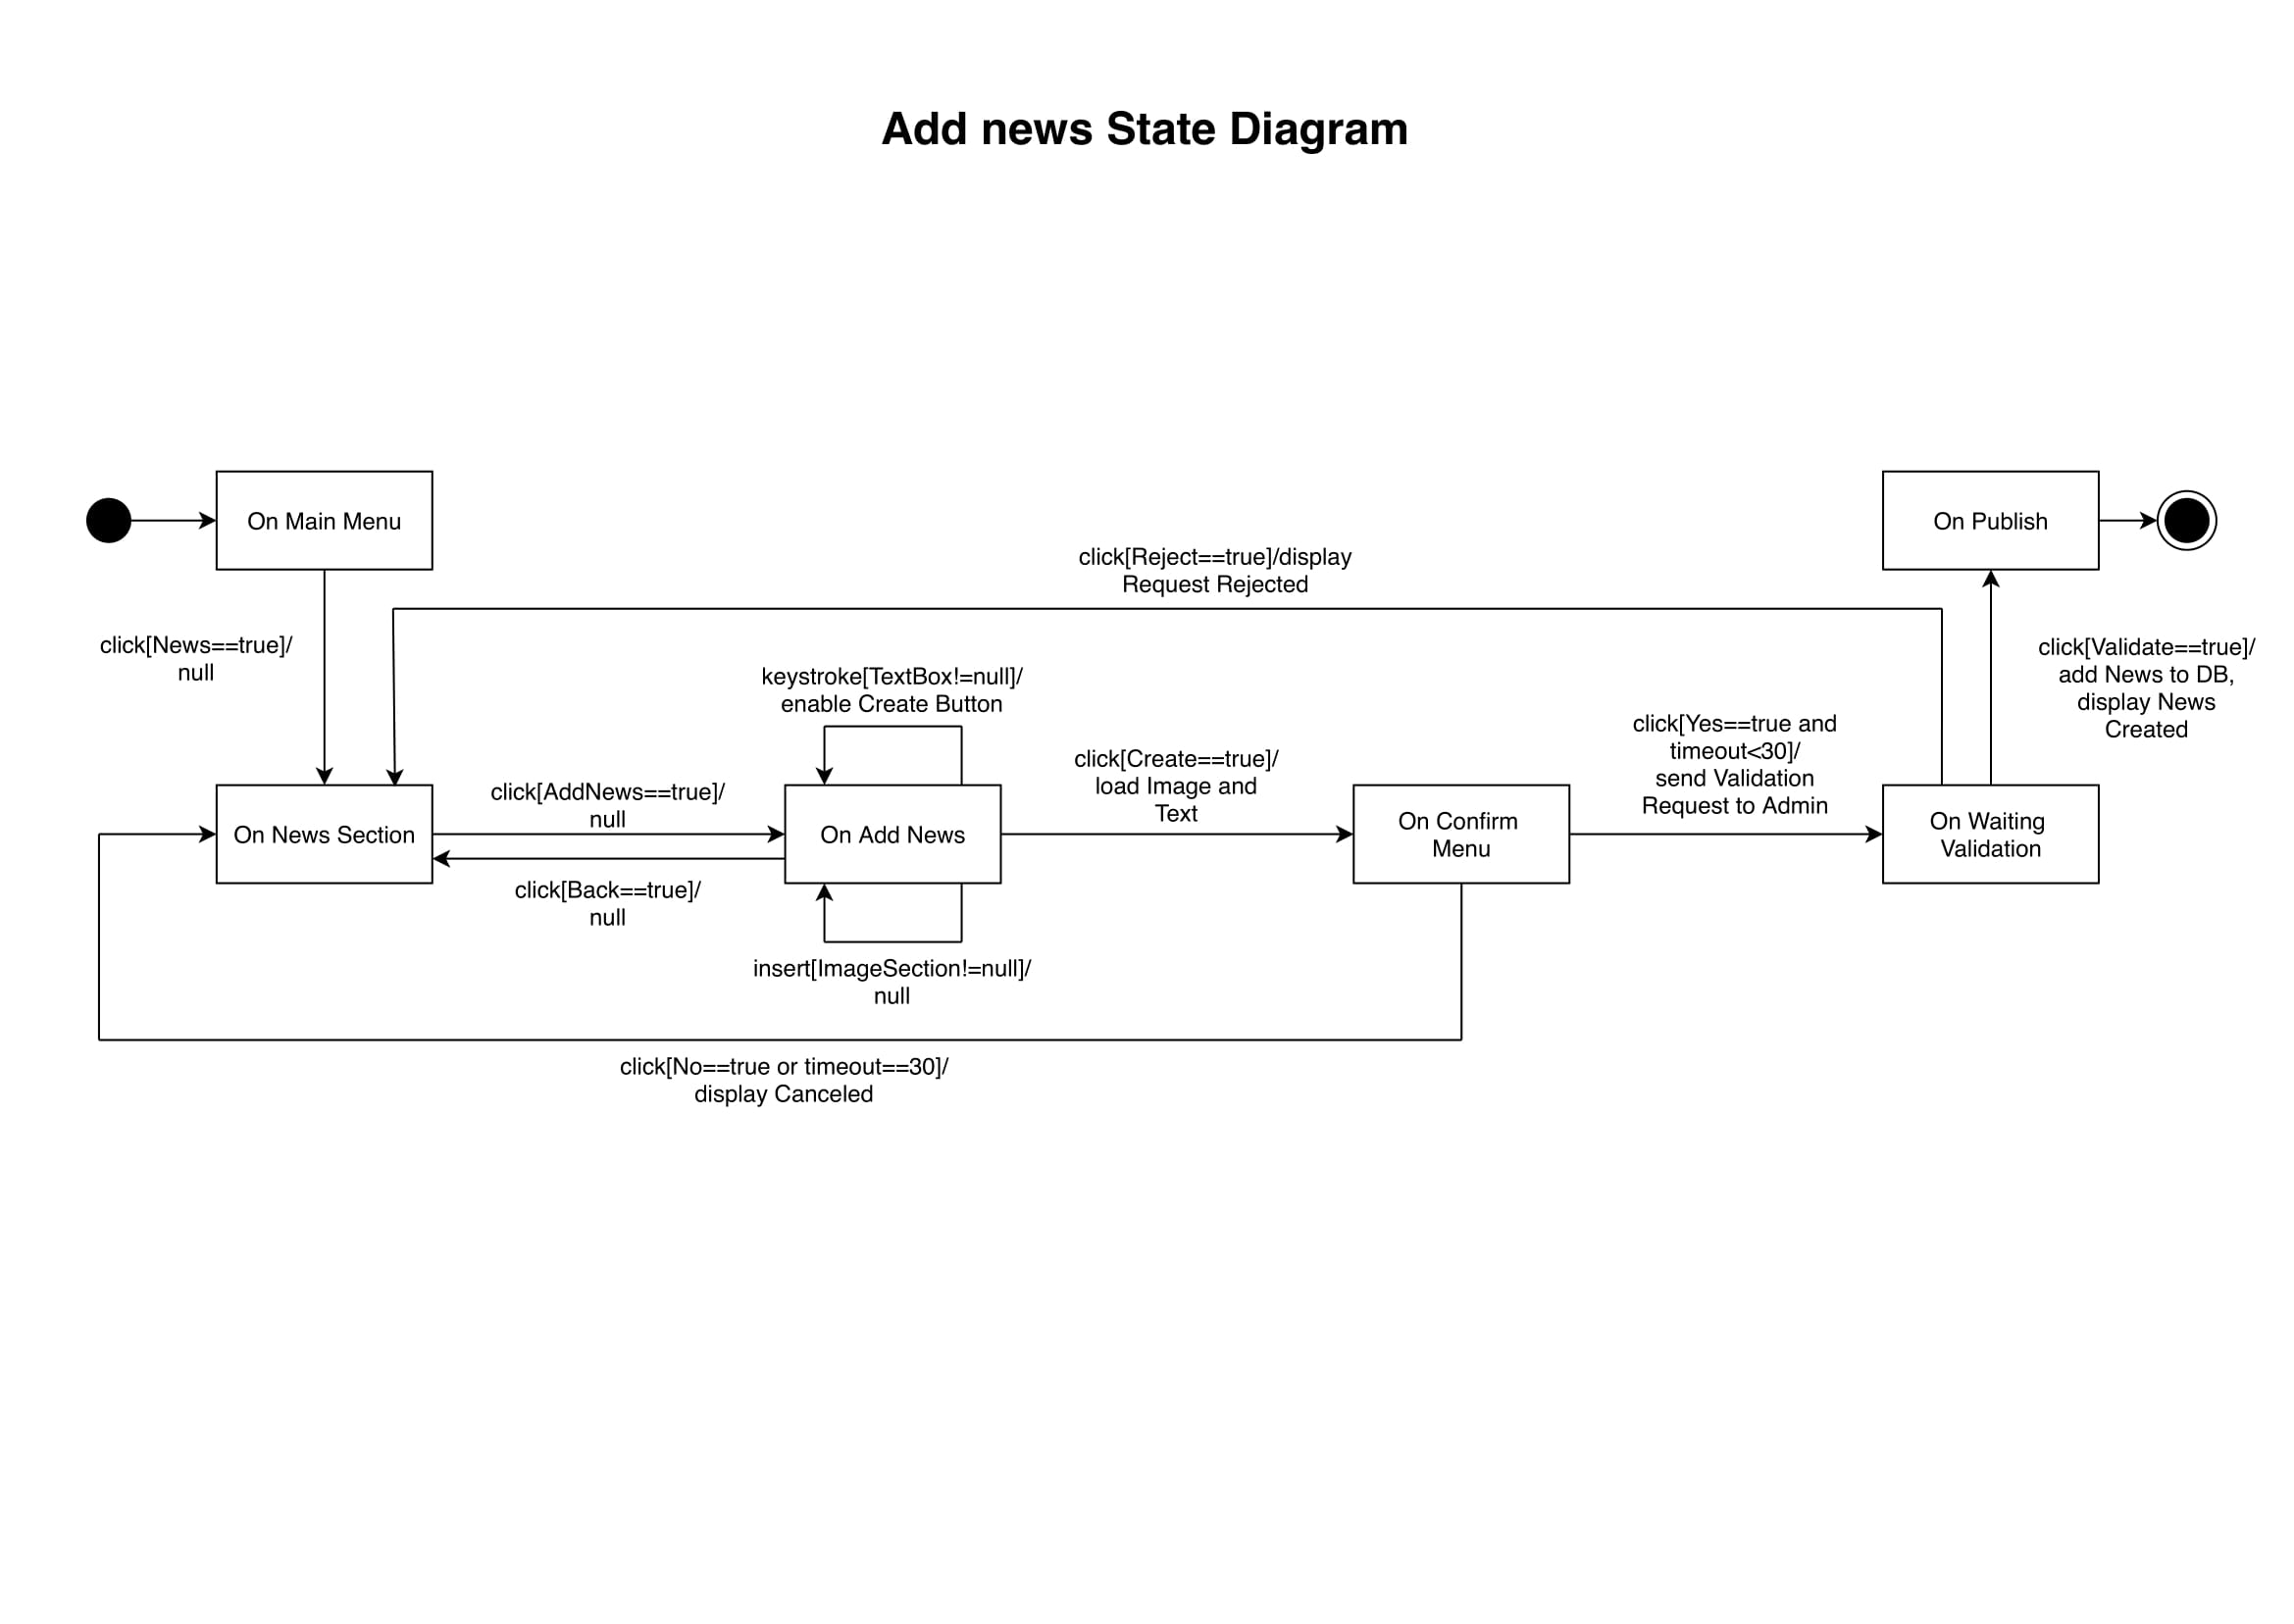
\includegraphics[scale=0.2]{SDFerri.jpg}
\subsection{Valeriani}
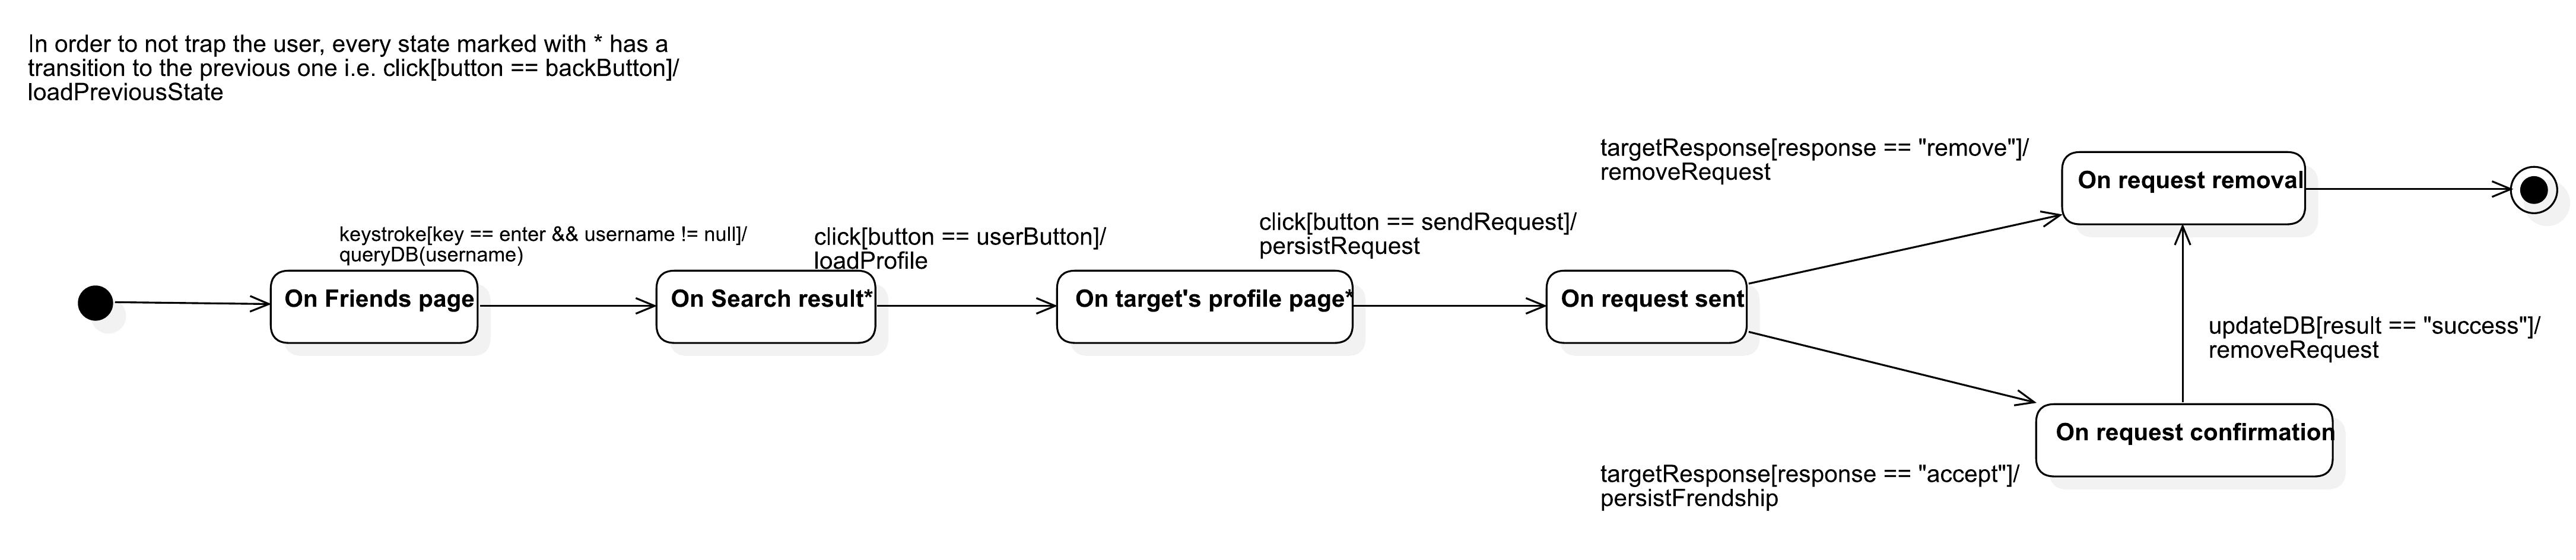
\includegraphics[scale=0.4]{SDValeriani.jpg}
\section{SonarCloud}
\paragraph{SonarCloud link} https://sonarcloud.io/dashboard?id=ferra-rally\_concert-scout
\end{document}